%!TEX root = thesis.tex 

\chapter{An Alternative Approach} \label{cha:An Alternative Approach}
\paragraph{}
If we take what we learned from the tools we described in Chapter \ref{cha:Towards a Better Web} and try to address the identified issues these tools have, we could greatly increase a user's experience when browsing the Web and create a better network of associative links between existing content. The one big challenge we face is to make the new tool as scalable as possible while also allowing it to expand and incorporate new features when the necessary technology arises.

\section{Separation of Concerns} \label{sec:Separation Of Concerns}
	\paragraph{}
	The one positive recurring feature that most of the tools implemented was the separation of the metadata from the actual content. This movement of separating all concerns has been making its way in multiple parts of the Web as well. Most HTML elements can have a style attribute attached to them. This attribute can be inlined into the HTML like so: \code{<div style="color:red">}. This will ensure all text within this \code{div} to be rendered in red. Suppose we wanted all our \code{div}'s text to be red we could create a style element in our HTML page like so: \code{<style type="text/css"> div\{color:"red";\}</style>}. This makes the maintenance of the page a lot easier. Instead of having to change all inline styling for each \code{div} element on the page, we can just change the inline style-tag's content to achieve the same effect. However, most sites consist of multiple HTML pages and not just a single one. If we wanted to change the styling of our \code{div}s over the entire website, we would still have to manually change all the HTML files to incorporate this change. This is of course cumbersome and error prone. To remedy this problem, cascading style sheets (CSS)~\cite{Etemad2011} were invented, separating the structure and content of the page from how the page should be styled. The content and structure is described by the HTML file, while the styling is defined in the CSS file. If we now include the CSS file on each of our web pages we can simply change the styling in the CSS file and the entire website would reflect this change. Since the introduction of CSS it has become a sort of taboo for websites to style their elements within the HTML structure and it is considered bad website design if some elements have embedded styling.
	\paragraph{}
	The same evolution is happening with JavaScript files as well, moving from inline \code{<script>} tags to JS files that can be included into the page.
	\paragraph{}
	It is strange however that web standards have not yet separated the linking from the content as well. Links between different resources are still embedded into the page by means of an anchor tag. If we separate this concern from the content as well, we can change, add or remove links from a web page with the same ease as we can change its styling. This technology, however, is not yet incorporated in the current HTML standard.
	\paragraph{}
	Most of the tools discussed in Section~\ref{sec:Existing Tools} already saw the benefits of separating the content from the linking metadata and therefore save the linking metadata in a separate local file or on a remote shared database.

\section{Link Filtering} \label{sub:Link Filtering}
	\paragraph{}
	The goal of the tool is to represent the saved metadata on a web page. As discussed in the previous chapter, we need to render this metadata in such a way that the page is still readable and usable by all users. So we need to device a strategy that allows us to render a large amount of metadata on the page, without cluttering it. We will now describe a couple of approaches we can take to achieve this goal.
		\paragraph{}
		The main problem when dealing with a multi-user system of this nature, is the amount of metadata that needs to be visualised. Previous tools could ignore this problem because they were intended to be used by either a single user, or a small group of users. So a seemingly obvious way to bypass the issue of an overfull page that is not usable by the users is to filter the metadata that is rendered to a manageable amount. There are a couple of ways we can go about how filtering the total amount of links to a manageable set that can be cleanly rendered on the HTML page without overwhelming the users.

	\subsection{User Specified} \label{ssub:User specified}
		\paragraph{}
		A simple, yet effective way to weed out the excessive, unneeded links is to have the users specify what data they are interested in. The users could for example change their options in the tool to specify that they are more interested in PDF files than videos. In the same way they could ask the system to filter out any metadata that is older then 2 months because they have most likely already heard about this information by then. By filtering in this way, they ensure that the new metadata stands out in the web page so they can easily see what new information is available for the topic.
		\paragraph{}
		The amount of parameters on which users can filter their metadata can be very large. But this introduces another issue. How will the tool keep up with all the new parameters of filtering data. It is infeasible to know all the different ways to filter the metadata in advance and even if we would know these parameters, the list would be so large that it would be cumbersome for a user to configure the tool so that it will represent its needs. Off course this problem can be bypassed by having the users create their own filtering parameters too. We can take the website Twitter.com as an example for this. On Twitter a user can specify an arbitrary tag that they are interested in and if someone else on Twitter posts a message that includes this arbitrary tag the users will be notified of this. This approach has proven to be very effective for classifying metadata~\cite{macgregor2006collaborative}. A similar approach can be taken to filter the metadata for the users based on their specified tags.
		\paragraph{}
		Even though the filtering of metadata can be done more or less in the same way as Twitter does it, we need to take into account that there can be a very large set of different tags. So telling the tool how to handle each specific tag is not viable. The users could create a default fall back in case there is no rule specified for a specific tag. This would solve the problem of having to specify too many rules. But this will also result in a lot of data being hidden from the user, even though they might have been interested in this information. Imagine the users configuring the tool in such a way that the tag \squote{OrbitalPhysics} needs to be rendered and nothing else. Because these tags are so arbitrary, there might be other users tagging their metadata with the tag \squote{Orbital\_Physics}. As we can see this will cause the metadata to be hidden for the user, so they are missing information that they actually wanted to find. Determining whether two different tags are in fact synonyms is quite a problem and requires additional semantic information~\cite{marchetti2007semkey}.
		\paragraph{}
		This problem stems from the fact that the tool is used by a large community. If there was a set of rules as to how a tag needs to be formatted this particular problem would be solved. But there are many more of these scenarios that can cause the system to fail and this would result in a user either seeing data they did not intend to see, or the users might not see some information that they actually did want to see. This technique for filtering the metadata is heavily reliant on the community's tagging rules.
		\paragraph{}
		To help mitigate this problem the tool can aid the users when they are tagging their hyperlinks. The tool can auto complete while the users are typing the tag they want to add. By showing the users already some of the suggestions it is easier to select one that is fitting. The tool could query the database to find out how many hyperlinks already exist containing this particular tag. If there are two different tags that are synonymous the users can see which of the two is used more often, and then follow this trend in their own hyperlinks.
		\paragraph{}
		When a user wants to share some information with the community by means of adding metadata to a website they need to fill in as much extra metadata as possible. If the users for example neglects to specify that the hyperlink they are adding points to a PDF file, many users that wanted to see this information will not get to see the links when they visit the web page because they might filter out any link that are not pointing to a PDF file. This means that the authoring of links or metadata has a lot of overhead and becomes significantly more difficult and time consuming for the users. Ideally the tool should automatically detect as much metadata as possible to fill in for the users.
		\paragraph{}
		Since we cannot know all the different filtering criteria when creating such a tool, we cannot enforce strict rules on how the authors of a hyperlink needs to tag their metadata. Because of this, the system will be very vulnerable to spammers and malicious users who can create links to fishing websites but they might tag the link as a relevant video or something similar.
		\paragraph{}
		So there are a couple of important drawbacks of this system, but it is not without benefits. The fact that a user can specify in a very fine-grained way what they are interested in is a significant benefit. These rules are also easily changeable if the users so desire. Suppose that users are currently working on writing a thesis and they are looking for interesting papers they can use as reference. At this moment the users are not interested if the same information is also available in the form of a YouTube video. However, when the users are not looking for these papers to refer to any more and they are merely looking for the information, they might be interested in these videos too. They can then go to the configuration of the tool and change the rules that specify which type of metadata needs to be rendered.
		\paragraph{}
		The fine-grained nature of the rules combined with the ability to change the rules on demand is a very powerful way to filter out unwanted links and match the needs of the user.

	\subsection{Community Based} \label{ssub:Community Based}
		\paragraph{}
		A different yet somewhat similar way to filter the amount of links to be rendered is by relying on the community as a whole to filter the unwanted links. If a link is created and posted on a website the community will then decide whether the link is relevant to the topic of the website or not. By allowing the users of the tool to up- and down-vote these links we can attach a score to each of the created links. This score can then be used to filter irrelevant metadata from the website. The users will be able to configure their tool to set a minimum score that a link needs to have in order for it to be rendered. A user that is only looking for the most accepted or popular links will set a fairly high threshold while other users might want to see more by setting the threshold lower.
		\paragraph{}
		In the scenario where the author of the metadata has neglected to fill in some information the community could also fix this problem. If the link is relevant, but the author forgot to specify that it links to a PDF file, other users might be allowed to fill in this information in their stead. This will ensure that the links that pass the evaluation of the community will have a certain degree of hygiene with which the community is satisfied. The previously described example where a link is tagged with \squote{Orbital\_Physics} but the community expects these type of links to be tagged with \squote{OrbitalFhysics} should not happen any more. Either the link will be down-voted because it was not complaint with the community's tagging rules or the metadata will be changed by the community to make it fit their standards.
		\paragraph{}
		The beauty of this system is the fact that it is self-regulating and very stable~\cite{moore2008evaluating}. The community will decide the rules and based on these rules, links will get rated. Spammers, who will create links that span multiple paragraphs will get down-voted because of that. If several links are created on the page that all point to the same resource, the community will replace the duplicates with a single hyperlink with multiple sources instead.
		\paragraph{}
		A second benefit is that the system is democratic. The eventual result of which links are rendered and which ones are hidden will be decided by the majority of the community. A single user that has a different believe then the community cannot force his viewpoint on the community, unless a large portion of the community shares that user's vision.
		\paragraph{}
		But this is also a big weakness of the system. If the majority of the users thinks a certain links is irrelevant it does not necessarily mean this is actually the case. And someone who is looking for this less popular information will not find it. The users could possibly set their threshold significantly lower to find the information they are looking for, but they will have to go through all the rejected metadata as well and this is time consuming and defeats the purpose of filtering the bad links in the first place. This problem will become especially noticeable when multiple large groups of users have different opinions about a certain topic~\cite{sumi2011edit}.
		\paragraph{}
		Another concern we could have with this system is the fact that it punishes new content. Suppose a couple of hundred links are already on the web page and they are all considered important and interesting. That means all of these links have received a significant amount of up votes by the community. When a user finds another source of relevant information they will create a new hyperlink to that resource. But since this is a new hyperlink it has not yet received any up votes, an will therefore not be rendered for any of the users browsing the website.
		\paragraph{}
		One way to solve this problem is to decrease the amount of votes for all existing links. All existing links will be decreasing in the amount of votes at the same rate. Therefore the relative difference in votes will stay the same. New links however will have a reasonable chance of getting noticed because they will start at a fixed value of votes that does not decrease over time.
		\paragraph{}
		But this opens up the issue of spamming again. Malicious users could keep creating new links on the web page and since all other links are diminishing in votes, eventually their new links will make it to the page for other users to be seen. So the system is not perfect and spamming will still be a possibility but the effect is a lot less prominent then it was in the previous discussed alternative.

	\subsection{Machine Learning} \label{ssub:Machine Learning}
		\paragraph{}
		The problem with community based approaches like the previous two suggestions are that they, well, depend on the community and the system only works as good as the community. In certain cases this approach has proved to be very beneficial, the Reddit\footnote{\url{http;//www.reddit.com}} community or the Stack Overflow\footnote{\url{http://www.stackoverflow.com/}} karma system have ensured the websites to be filtered of malicious content quite effectively, while providing the users with quick access to the information they are looking for. However this is not always the case and for smaller communities these converging situations may not be achievable. Since we are enhancing the Web as a whole, we have to take into account the less popular parts of the Web as well. In these parts there will also be malicious users but the communities for these topics could be to small so there will be less people to correct these wrongs. The previous mentioned systems will not perform as well as for large communities.
		\paragraph{}
		Another approach may be to create a user profile based on the links a user previously followed. If the users, for example, rarely follow links that point to blog posts, the system will learn that these type of links might not need to be rendered on future pages. If we allow the users to steer the machine learning into a certain direction, by flagging certain types of links to be unwanted, the amount of metadata that is rendered can be reduced further. This method can in some way mimic the first suggestion where each user configures the tool themselves. The difference is that there is will be less overhead for the authors of links. They can still just create hyperlinks without having to fill in any additional metadata and the system will then have its own rules to determine the type of the link and detect whether or not a user might be interested in this link.
		\paragraph{}
		If the users could steer the system with suggestions of what links it should not render we can create a better filter. However it is difficult to allow links to be rendered once the system had already decided not to render them. In essence this is not a problem, the issue is that the users will not know that certain possibly interesting information is present because the algorithm blocked it from being rendered. So even if the users wanted to see this information they will never get the chance to let the system know. They could of course change their settings and re-render already blocked links, but that would defeat the purpose of the filter.
		\paragraph{}
		The same problem is also present with big search engines that try to optimize the search results based on some generated user profile. Instead of showing all results in an unbiased way, some results that are deemed uninteresting by the system will not be rendered for this particular user. In essence a user will be wrapped in a sort of information bubble, where all the information that is in the bubble will be available, but all the other information will never be shown to the user, even if they might find it interesting~\cite{pariser2011filter}.
	\subsection{On Demand} \label{ssub:On Demand}
	\paragraph{}
	As stated before the problem lies in the fact that there are too many links to be rendered on the page. This would make the web page cluttered and unusable by the reader. Any interesting metadata that is available cannot be found in the sea of data that is being created. One way to limit the amount of metadata that is being rendered is to render only the plain, unaltered page at first. The page would just be the blank vanilla page as the author has intended it to be. We could then provide the metadata on demand of the users. For example, when the users highlight a part of the text the tool sends a request to the server fetching all the metadata for the content that lies within the selection. On this selection the tool will then render the fetched metadata.
	\paragraph{}
	The benefit is that we do not clutter the page beforehand. And if the reader is not interested in getting more information about certain parts of the document, they will not be bothered with additional links. If they find a specific part of the document that they want more information about, they can easily get this on demand by selecting that part of the document.
	\paragraph{}
	It is however still possible that the selection of the users contains so many links that this small selection is already cluttered with links. The users can then narrow their selection to specify more clearly the topic they want more information about.
	\paragraph{}
	The benefit of this approach is also its downside. The fact that the users need to prompt the system for information can be cumbersome. The users might be reading a part of an article, but the community has provided hyperlinks to articles proving the falsity of this article. Unless the reader actually selects the paragraph that contains this hyperlink they will not see this additional information.
	\subsection{Conclusion} \label{ssub:Conclusion}
	\paragraph{}
		All of the discussed techniques for filtering links have benefits and drawbacks. Most of them can be used in unison reducing their drawbacks and increasing their combined benefits. For example, we can dynamically load content by making use of the users' selection but after the links are requested we can filter this data based on the users' preferences, or profile. On top of this we can even make a default filtering based on the opinion of the community to get a better selection of the relevant hyperlinks. The community could also mark some metadata as \squote{Must See} so that these links will be rendered even if the users did not select that part of the document, reducing the chance of missing vital information.
		\paragraph{}
		In conclusion all of these techniques will help reducing the amount of links that need to be rendered, but to have the most benefit it is advised to create a system that is a combination of these techniques.
\section{Link Rendering} \label{sub:Link Rendering}
	\paragraph{}
	Now that we have established some ways of reducing the amount of links that need to be rendered, we can discuss how to render the selected, relevant links. This step of the process is crucial to provide the users with a usable system that helps with finding relevant information, instead of working against the user. If the visualisation is suboptimal the information that was selected in the previous step will not be presented to the users in an optimal way and makes the tool as a whole suboptimal. Therefore we now describe a couple of different approaches that can help in the visualisation of the selected metadata.
	\subsection{In Place} \label{ssub:In Place}
	\paragraph{}
	All of the previously discussed tools render the metadata on top of the actual content. They either add small indicators that notify the users of the presence of a hyperlink, or the tool highlights the text that is associated with the link. This technique is rather easy to implement, but poses a visual issue. Even with all the work of reducing the amount of metadata to be rendered, it is still possible that a single word is the source of multiple links. Suppose that NASA is mentioned in a sentence as one of the keywords. One user might want to link to NASA's own homepage, while another user chooses to link to the Wikipedia page with more information about NASA. Both sources are relevant to the context, but it is hard to distinguish the two links if they are rendered on the same word.
	\paragraph{}
	Many tools opted for a colour code approach to distinguish between these overlapping links. This will help when two links are overlapping. The tool could for example highlight the first of link in red and the second one in green. To show the users that the overlapping part contains two links, it could highlight the top in red and the bottom in green. This of course does not scale well if more then two links are overlapping.
	\begin{figure}[h]
		\centering
		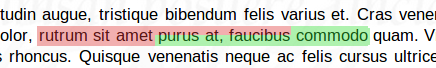
\includegraphics[width=\textwidth*4/5]{idealtool/overlapping.png}
		\caption{Overlapping links visualisation}
	\end{figure}
	\paragraph{}
	Other tools introduced layers of annotations. A link would be designated to a specific layer based on the metadata the author of the link provided. The tool will allow the users to toggle the rendering of specific layers to their liking and each of the layers will be colour coded. This does not scale well with a large amount of links either. And disabling layers will not solve the problem when two links on the same layer are overlapping.
	\begin{figure}[h]
		\centering
		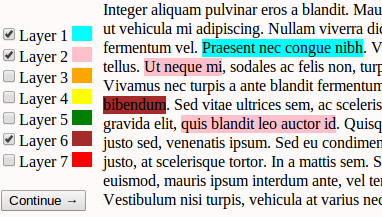
\includegraphics[width=\textwidth*4/5]{idealtool/layers.png}
		\caption{Layered visualisation}
	\end{figure}
	
	\paragraph{}
	A third option some of the tools used was to add an icon after the text on which a link exists and if multiple links are available on the same part of the text they would add additional indicators. But this would soon become an issue as well when too many links were present and therefore many icons needed to be added behind the text. A second down side was that the start of a link could not be indicated in this way.
	\begin{figure}[h]
		\centering
		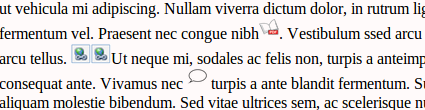
\includegraphics[width=\textwidth*4/5]{idealtool/icons.png}
		\caption{Using indicators for hyperlinks~\cite{bottoni2004madcow}}
	\end{figure}
	\paragraph{}
	Instead the tool could add icons after parts of the text that contain hyperlinks and also add an indicator of how many links are in this location. If a user clicks on the indicator a menu will open, containing the different hyperlinks. This approach will limit the amount of indicators to a minimum but does not yet address the problem of omitting the start of the link.
	\paragraph{}
	A big benefit of this approach is that the icons will replace the blue underlined text as a metaphor for the presence of a hyperlink. This is compatible with the users' way of browsing the Web, so using this technique will not drastically change how they will interact with online information.
	\paragraph{}
	Normally the destination of a hyperlink, as well as most of the other metadata, is hidden from the user. Users will just click on the blue underlined text and expect to be redirected to the associated page. Users following the link trust the author of this link that it will redirect them to a page that is meaningful to the context in which the link occurred. However in the scenario where multiple links exists on the same content a user will be prompted with a menu of links to choose from. This may not seem like a big issue, but the fact that the users need to choose between several options means that the tool must provide enough information about the different hyperlinks. The question then arises is: \dquote{How will the tool visualise the different hyperlinks in such a way that the users are presented with enough information to make an informed decision about which link to follow?}
	\subsection{Separated} \label{ssub:Separated}
	\paragraph{}
	A radically different approach of rendering all the metadata on a page is by separating the content of the page from the visualisation of the metadata. Instead of rendering the links between or on the text, the tool will create a designated area in the browser under the window in which the web page is rendered. In this area only the metadata will be rendered.
	\paragraph{}
	This approach has a couple of major benefits. The first important one is that this method overcomes the limit of the two dimensional canvas that the web page offers us. History and common web browsers have indoctrinated the idea of rendering a link on top of its context. This makes sense since an important dimension of the hyperlink's metadata is the location on which it was created. Because the simple links HTML offers us do not have a lot of dimensions there was never really a need to use different dimensions of the metadata. With the new method of creating hyperlinks many new dimensions get introduced. All of these dimensions are equally important in different scenarios. So limiting ourselves to the structure of the web page is only one way of using a single dimension to render the metadata.
	\paragraph{}
	If we decide to render the metadata in a separate window we can use all the different interesting dimensions to render the data. If we represent each web page or website as a single node in a large graph we can represent the hyperlinks as edges between these nodes. This representation lends itself exceptionally well to visualisation and using this approach we can take advantage of all the recent work in the active field of data visualisation.
	\begin{figure}[h]
		\centering
		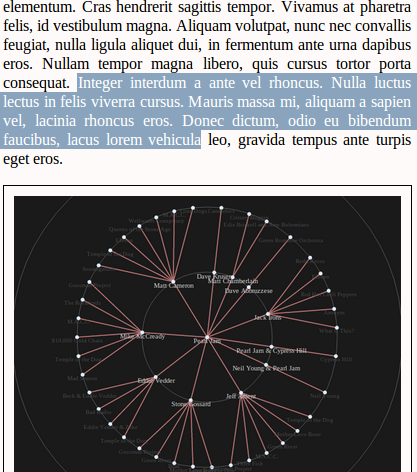
\includegraphics[width=\textwidth*4/5]{idealtool/graph.png}
		\caption[test]{Graph visualisation of metadata in selection based on JavaScript InfoVis Toolkit\footnotemark}
	\end{figure}
	\paragraph{}
	The tool will also be able to take advantage of the extra metadata that is added to the hyperlinks. Any dimension that is introduced by the metadata can be used to help with the visualisation. Nodes can be made bigger based on the popularity of the associated web page and colours can be added to represent the domain of the page. The relative positioning of the nodes can also be used to visualise another dimension of the metadata.
	\footnotetext{\url{http://philogb.github.io/jit/}}
	\paragraph{}
	Depending on the question at hand the tool can also change the visualisation from a graph to another more appropriate format. When a user wants to find a website with a strong correlation to the current page the different domains can be rendered on a radial representation as shown in figure \ref{pic:radial2}. In this image we can see 6 different domains represented by the letter A through~F. The ribbon connecting the various domains represent how strongly the two domains are linked together. As we can easily see from this one image is that the domain F is most strongly connected to the domain C since almost half of the existing links point to this domain. This information is quickly accessible for the users because of the way the metadata is presented.
			\begin{figure}[h]
				\begin{centering}
				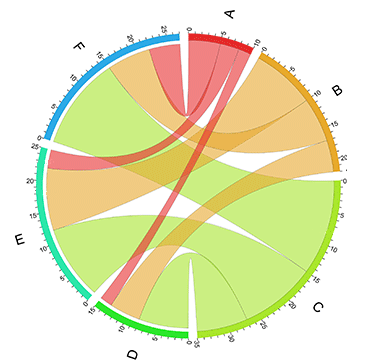
\includegraphics[width=\textwidth*4/5]{idealtool/radial2.png}
				\caption[test]{Radial Ribbon Visualisation based on d3.js\footnotemark}
				\label{pic:radial2}
				\end{centering}
			\end{figure}
	\paragraph{Zoomable}
	Because we are rendering a plain data graph we can hide a lot of complexity of the graph in large nodes. This view will provide the users with a general overview of the linking structure on the web page. Zooming in on certain parts of the graph could expand these nodes and show more detail for that particular section. For example, we could create a big node entitled \dquote{YouTube}. The size of the node will be defined by the amount of links pointing to the YouTube domain. This size will already give an overview to the users about how much information is available as video fragments. If the users are interested in a video clip about the topic they can zoom in on this one big node to show more detail. When the zoom level is sufficient the node will expand showing the different videos the page links to. This is a fairly simple example but zoom functionality can be a powerful tool to initially hide a lot of complexity for the user.
	\footnotetext{\url{http://d3js.org}}
	\paragraph{Searchable}
	The content of the graph can also easily be filtered based on some search criteria specified by the user. If the metadata is tagged as described in Section~\ref{sub:Link Filtering} the users can use these tags to filter the metadata on request. If the users are for example looking for scientific papers about orbital physics they can search the graph with these keywords as well as search for hyperlinks that are tagged as PDF. All nodes that do not fit their search criteria will be removed from the visualisation. The benefit is that the graph will still represent the structure of the metadata after the unwanted links are removed from it.
	\paragraph{}
	All of the previously mentioned filtering techniques can also be used with this visualisation. The on demand filtering described in Section \ref{ssub:On Demand} can easily be adapted to the separated view. When the users select a part of the text in the original web page the graph view will be updated in such a way that the nodes and edges represent the metadata that is found within the user's selection. Using this technique the users can easily find out if there is more information available about the context they have selected. This kind interactivity between the users' actions and the visualisation is a very powerful way of helping the users find what they are looking for.
	\paragraph{}
	Visualising the metadata in a different view that is completely separated from the structure of the web page has many benefits but there is one major drawback to this approach. The currently established metaphor of the presence of a hyperlink will be completely removed from the web page. The users can no longer look at the content of a web page and based on the blue underlined text see whether a link exists on this part of the text. And even though this may not seem like a big issue the users who have already established a way of browsing the web that works for them, will have a hard time adapting to any other way of working.
	\paragraph{}
	The users will have to keep an eye on two separated views that render two different aspects of the same content. In one frame the content is visible, while the other frame will only show the metadata. This can be confusing for new users and cause some frustration. Interaction with the metadata view could seem very detached from the web page and users will have to interact with two different views at the same time, increasing the overhead for the end user. All these effects are notable drawbacks to this approach and they should not be ignored lightly. Therefore a clear interface design needs to be established to make it easier for new users to use the tool without feeling lost because of the detachment.

\section{Link Authoring} \label{sec:Link Authoring}
\paragraph{}
Up until now we only discussed ways to visualise and filter already existing metadata. We did not yet touch the subject of how we will allow users to author their own metadata. Because we are introducing a more complex mechanism of linking resources together, it is obvious that conventional methods of creating hyperlinks will no longer apply.
\paragraph{}
In most existing tools, the users are provided with a tool bar with which they can use the authoring functionality the tool provides. Clicking a button on the tool bar will open a dedicated window for authoring. In this window the users are prompted for all additional metadata they want to provide. Typically the users are allowed to create a source selection by highlighting some text on the current page. And when the authoring window opens they are asked to input a destination URL for their new hyperlink.
\paragraph{}
Some of the tools allow the users to open new tabs, in which they can open different web pages. And when a user is authoring a hyperlink, the tool allows them to click on a tab instead of having to type the URL themselves. However, these tools do not allow the users to specify a destination selection so the authoring of the hyperlinks does not allow the users to take advantage of the full potential of the enhanced linking mechanics.
\begin{figure}[h]
	\centering
	\begin{subfigure}[b]{\textwidth*2/5}
		\centering
		$\vcenter{\hbox{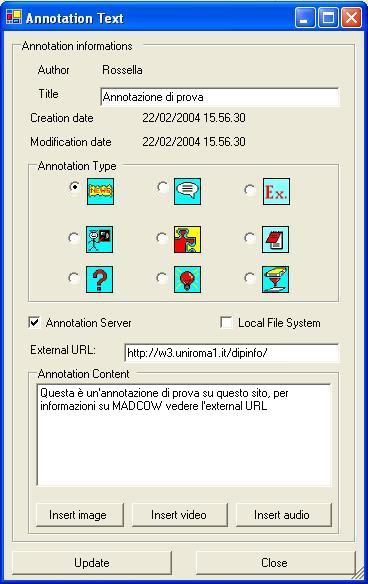
\includegraphics[width=\textwidth]{idealtool/authoring.png}}}$
	\end{subfigure}
	\begin{subfigure}[b]{\textwidth*2/5}
		\centering
		$\vcenter{\hbox{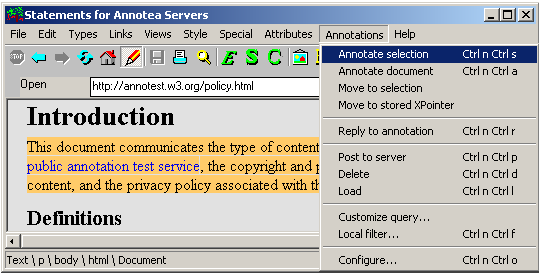
\includegraphics[width=\textwidth]{idealtool/authoring2.png}}}$
	\end{subfigure}
	\caption{Examples of authoring}
\end{figure}
\paragraph{}
We want to allow the users to author hyperlinks by navigating to the source web page and selecting the desired content. The users will then open a second tab or window in which they will navigate to the destination web page and select the content to which the link will point. Having both these selections in place the users will press a button in the tool bar that opens a window prompting them for more information. The difference is that the users are allowed to link to a specific part of a document instead of pointing to the document as a whole. This will add more flexibility and detail to the links resulting in a better experience for users looking for more information.
\paragraph{}
A third approach is to add functionality to the tool bar that allows the users to specify what role their current selection plays in the hyperlink. When the users select a part of the text they can press either one of two buttons. One will add the selection to the sources of the link, while the other button adds the selection to the destinations. This allows the users to easily construct hyperlinks with multiple sources and multiple destinations.
\paragraph{}
Each of the destinations are selections, so following a link will refer the users to the intended part of the linked document, instead of just the document as a whole. When finished the users will press a third button finishing the selection process and the tool will again prompt for more metadata, such as additional tags or comments.
